
% Tecator WMaxTwin section.  Generated by tecator_wmaxtwin_study.py.

\section{Tecator spectroscopy: a functional-regression example}

The Tecator data provide a natural real-data test bed for multiscale splitting in
functional regression.  Each observation is a near-infrared absorbance spectrum
measured on chopped meat over the wavelength range 850--1050 nm, together with
laboratory measurements of moisture, fat, and protein content.  We use fat
percentage as the scalar response and the absorbance spectrum as the functional
predictor.  Following the original interpolation protocol, the first 172 samples
are used as a calibration set and samples 173--215 are reserved as an external
test set.  The remaining extrapolation samples are not used in this comparison.

The functional regression model is a wavelet-ridge scalar-on-function regression.
The 100-channel spectra are linearly interpolated to 128 equally spaced grid
points, centered and scaled using the calibration sample, and represented in an
orthonormal Haar wavelet basis.  For a maximum retained resolution $j_{\max}$,
the model has the form
\begin{eqnarray}
Y_i &=& \alpha + \sum_{\ell \in {\cal I}(j_{\max})} b_\ell c_{i\ell} + \varepsilon_i,
\end{eqnarray}
where $c_{i\ell}$ are wavelet coefficients of the $i$th absorbance curve and
${\cal I}(j_{\max})$ contains the scaling coefficient and all detail
coefficients up to scale $j_{\max}$.  The ridge penalty and the scale cutoff
$j_{\max}$ are selected by an internal train-validation split of the 172
calibration samples.  After tuning, the selected model is refit on all 172
calibration samples and evaluated once on the 43 external test samples.

The split comparison uses train-validation sizes 129 and 43, matching the
original calibration-monitoring division.  We compare Random splitting, SPlit,
Twinning, DUPLEX, MaxTwin, and WMaxTwin.  In this implementation, MaxTwin forms
greedy nearest-neighbor pairs under the raw functional geometry and sends one
member of each pair to validation and the other to training.  WMaxTwin is a
nested multiscale extension of MaxTwin.  Let
\begin{eqnarray}
D_0^2(i,i') &=& \|X_i-X_{i'}\|_2^2
\end{eqnarray}
be the standardized raw-curve distance and let
\begin{eqnarray}
D_w^2(i,i') &=& \sum_{j=1}^J w_j \sum_k
\left(d_{ijk}-d_{i'jk}\right)^2
\end{eqnarray}
be a scale-weighted wavelet distance.  The nested WMaxTwin distance is
\begin{eqnarray}
D_\gamma^2(i,i') &=& (1-\gamma)D_0^2(i,i')+\gamma D_w^2(i,i'),
\qquad 0\leq \gamma\leq 1.
\end{eqnarray}
Thus ordinary MaxTwin is exactly the special case $\gamma=0$.  The added
wavelet geometry does not replace MaxTwin; it only perturbs MaxTwin toward scale
features that are relevant for the functional regression problem.

For the Tecator spectra, the scale weights are estimated from the calibration
sample only by the average squared marginal correlation between the fat response
and the wavelet coefficients at each scale,
\begin{eqnarray}
w_j &\propto& {1\over |{\cal K}_j|}
\sum_{k\in {\cal K}_j} \widehat{\operatorname{Cor}}^2(d_{ijk},Y_i),
\qquad \sum_j w_j=1.
\end{eqnarray}
This makes WMaxTwin mildly supervised, but the external test sample is never
used in constructing either the split or the weights.  The estimated weights in
this run were
\begin{center}
\begin{tabular}{rr}
\hline
scale $j$ & weight $w_j$ \\
\hline
1 & 0.008 \\
2 & 0.232 \\
3 & 0.107 \\
4 & 0.173 \\
5 & 0.154 \\
6 & 0.163 \\
7 & 0.162 \\
\hline
\end{tabular}
\end{center}

Table~\ref{tab:tecator-wmaxtwin} reports the results over repeated internal
splits.  The external test RMSE is measured in fat-percentage units.  The table
should be read as a validation-sensitivity comparison, not as a claim that any
one split is uniformly optimal.  The scientifically important diagnostic is
whether the nested WMaxTwin path improves on, or at least stabilizes, the
ordinary MaxTwin case $\gamma=0$.

\begin{table}[t]
\centering
\caption{Tecator functional regression.  Results are averaged over repeated
internal calibration splits.  The model is refit on all 172 calibration samples
after tuning and evaluated on the fixed 43-sample external test set.}
\label{tab:tecator-wmaxtwin}
\begin{tabular}{lrrrrr}
\hline
split & mean $\widehat{j}_{\max}$ & median $\widehat\lambda$ & mean val. MSE & mean test RMSE & sd test RMSE \\
\hline
Random & 6.50 & 0.131 & 5.5354 & 2.1826 & 0.4274 \\
SPlit & 6.00 & 0.00215 & 3.6737 & 3.2710 & 0.0000 \\
Twinning & 6.75 & 0.00608 & 2.7491 & 2.6714 & 0.9449 \\
DUPLEX & 7.00 & 21.5 & 21.7741 & 2.9433 & 0.0000 \\
MaxTwin & 6.75 & 0.0001 & 1.7609 & 3.3972 & 1.2224 \\
WMaxTwin $\gamma=0.10$ & 6.88 & 0.000464 & 2.3770 & 2.4301 & 0.5423 \\
WMaxTwin $\gamma=0.25$ & 7.00 & 0.0234 & 2.2809 & 2.2223 & 0.5205 \\
WMaxTwin $\gamma=0.50$ & 6.88 & 0.0234 & 2.6657 & 2.2577 & 0.4951 \\
WMaxTwin $\gamma=0.75$ & 7.00 & 0.000282 & 2.1997 & 2.5587 & 0.6828 \\
WMaxTwin equal $\gamma=0.25$ & 7.00 & 0.000282 & 2.3036 & 2.7394 & 0.5059 \\
\hline
\end{tabular}
\end{table}

Figures~\ref{fig:tecator-spectra}--\ref{fig:tecator-gamma} summarize the
experiment.  The spectra show smooth global structure but also local wavelength
regions in which fat-content groups separate.  This is precisely the setting in
which raw Euclidean geometry may be dominated by broad baseline variation, while
a multiscale perturbation can emphasize wavelength-local contrasts.  The scale
weight figure gives a direct diagnostic of whether the response is primarily
smooth, primarily local, or genuinely multiscale.  The selected tuning parameter
figures quantify validation sensitivity, and the nested $\gamma$ path checks
whether WMaxTwin improves on the raw MaxTwin endpoint.

\begin{figure}[t]
\centering
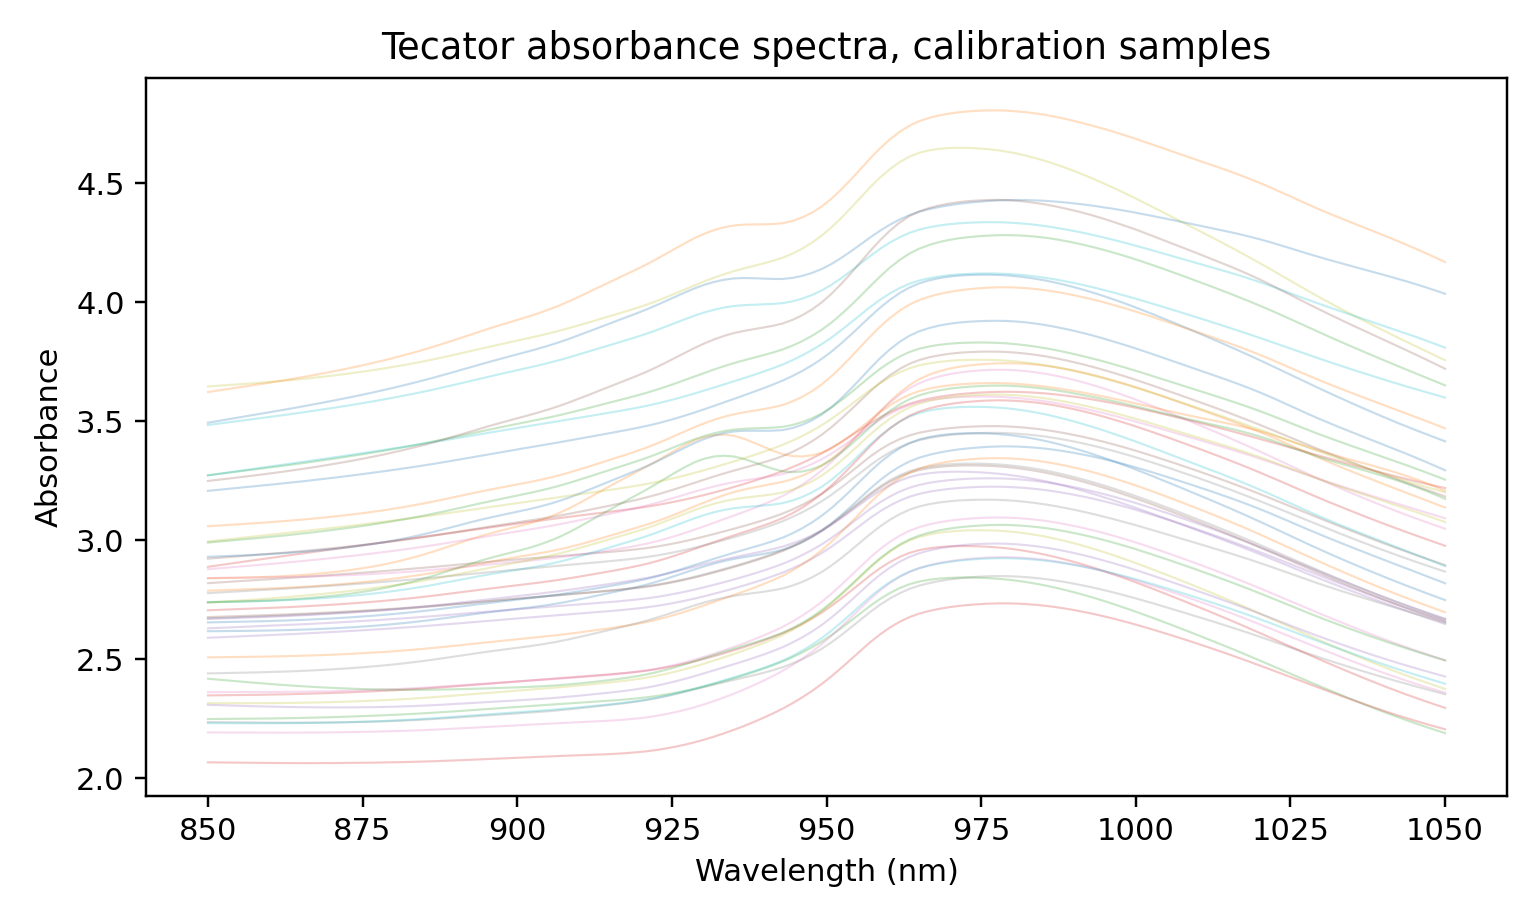
\includegraphics[width=.80\textwidth]{fig1_tecator_spectra.png}
\caption{Tecator absorbance spectra for calibration samples.}
\label{fig:tecator-spectra}
\end{figure}

\begin{figure}[t]
\centering
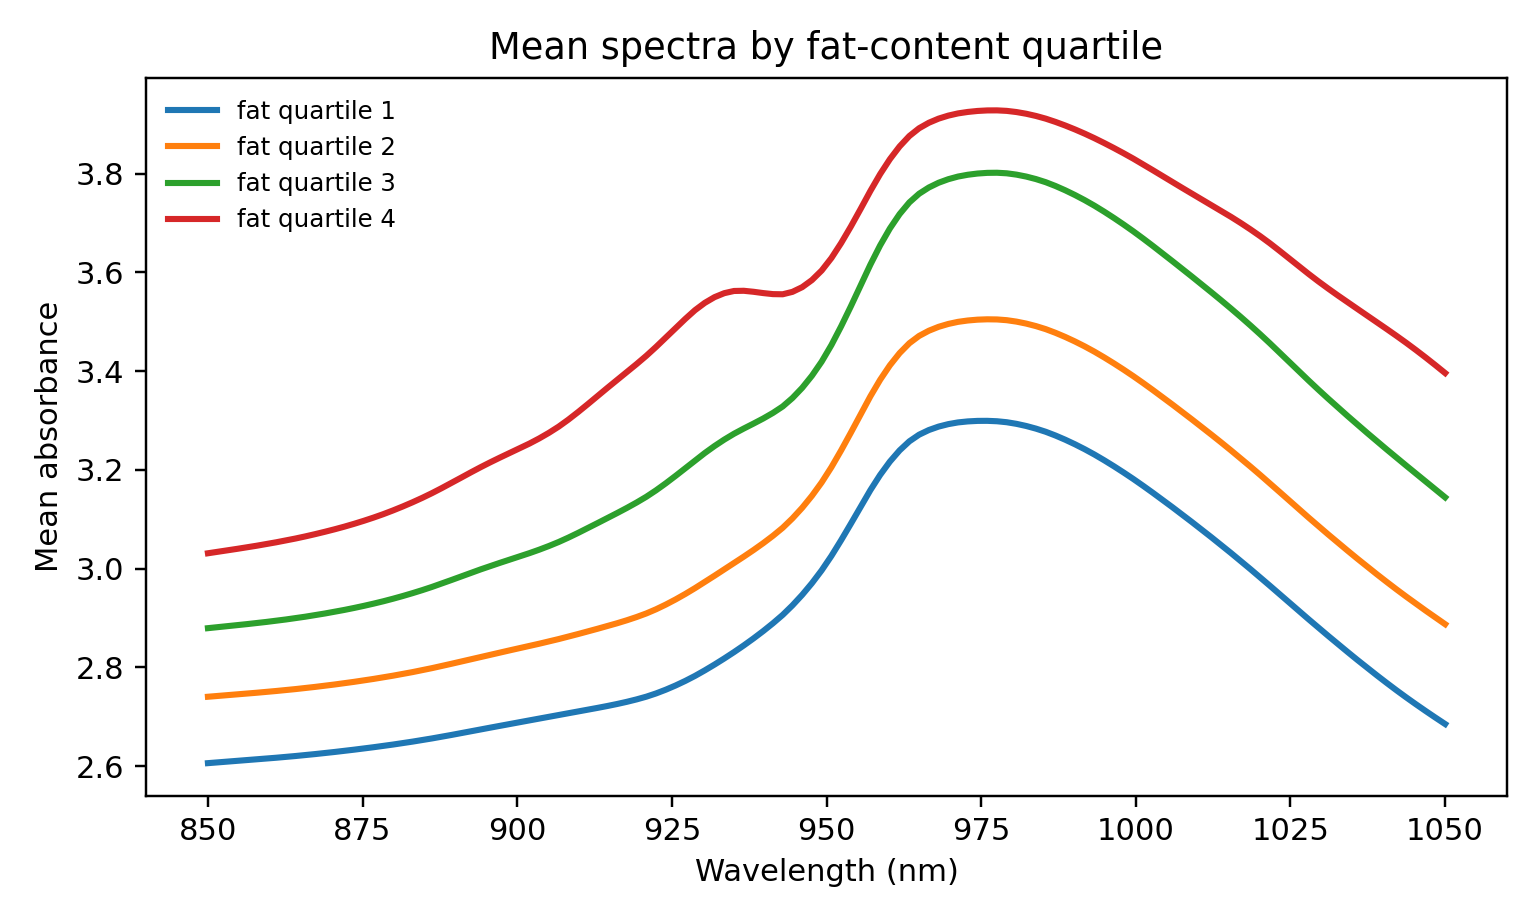
\includegraphics[width=.80\textwidth]{fig2_quartile_mean_spectra.png}
\caption{Mean absorbance spectra by fat-content quartile.  Separation of the
quartile means suggests that predictive information is not purely global; local
spectral regions also contribute.}
\label{fig:tecator-quartiles}
\end{figure}

\begin{figure}[t]
\centering
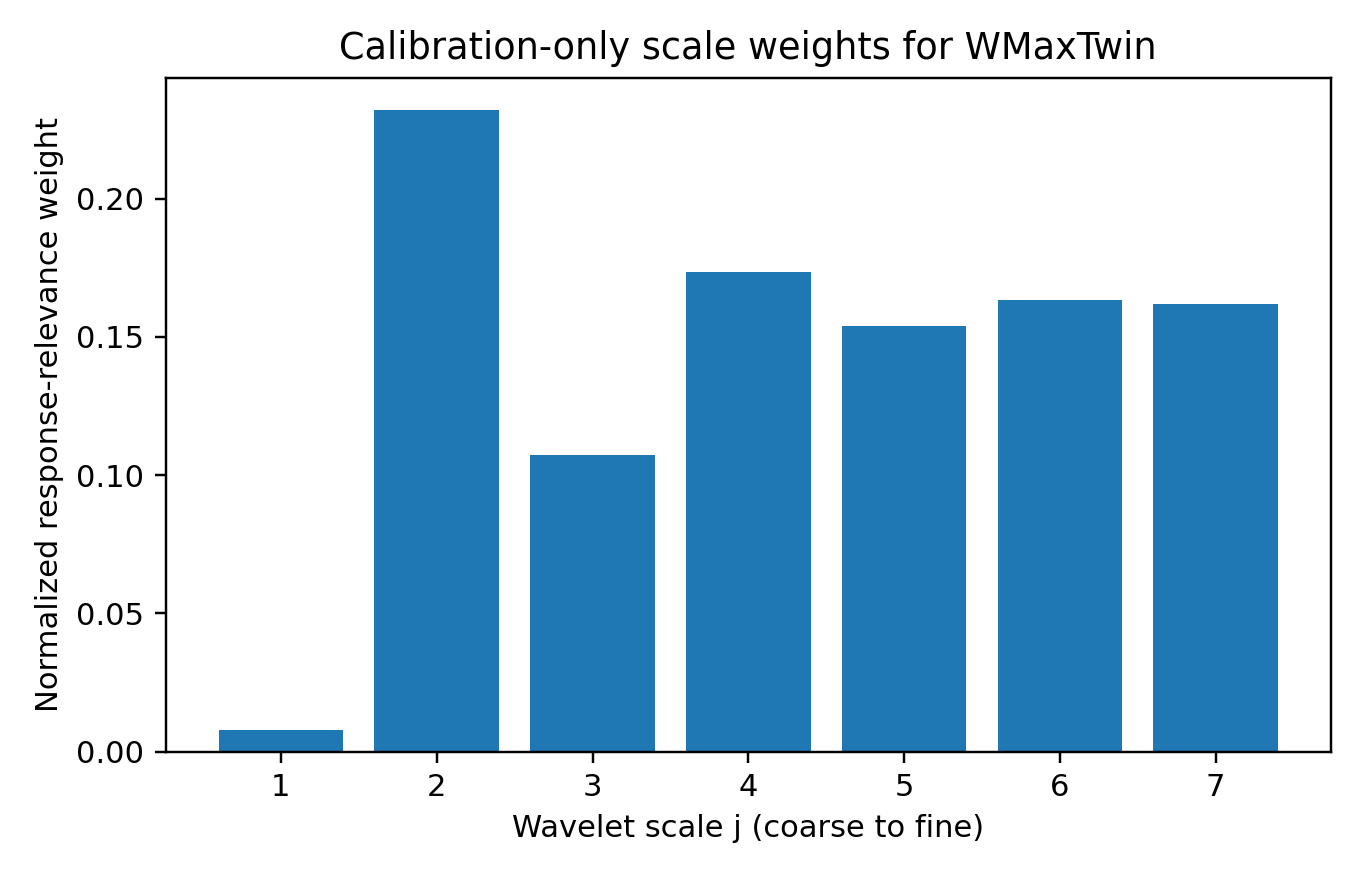
\includegraphics[width=.72\textwidth]{fig3_response_scale_weights.png}
\caption{Calibration-only wavelet scale weights used in the WMaxTwin geometry.}
\label{fig:tecator-weights}
\end{figure}

\begin{figure}[t]
\centering
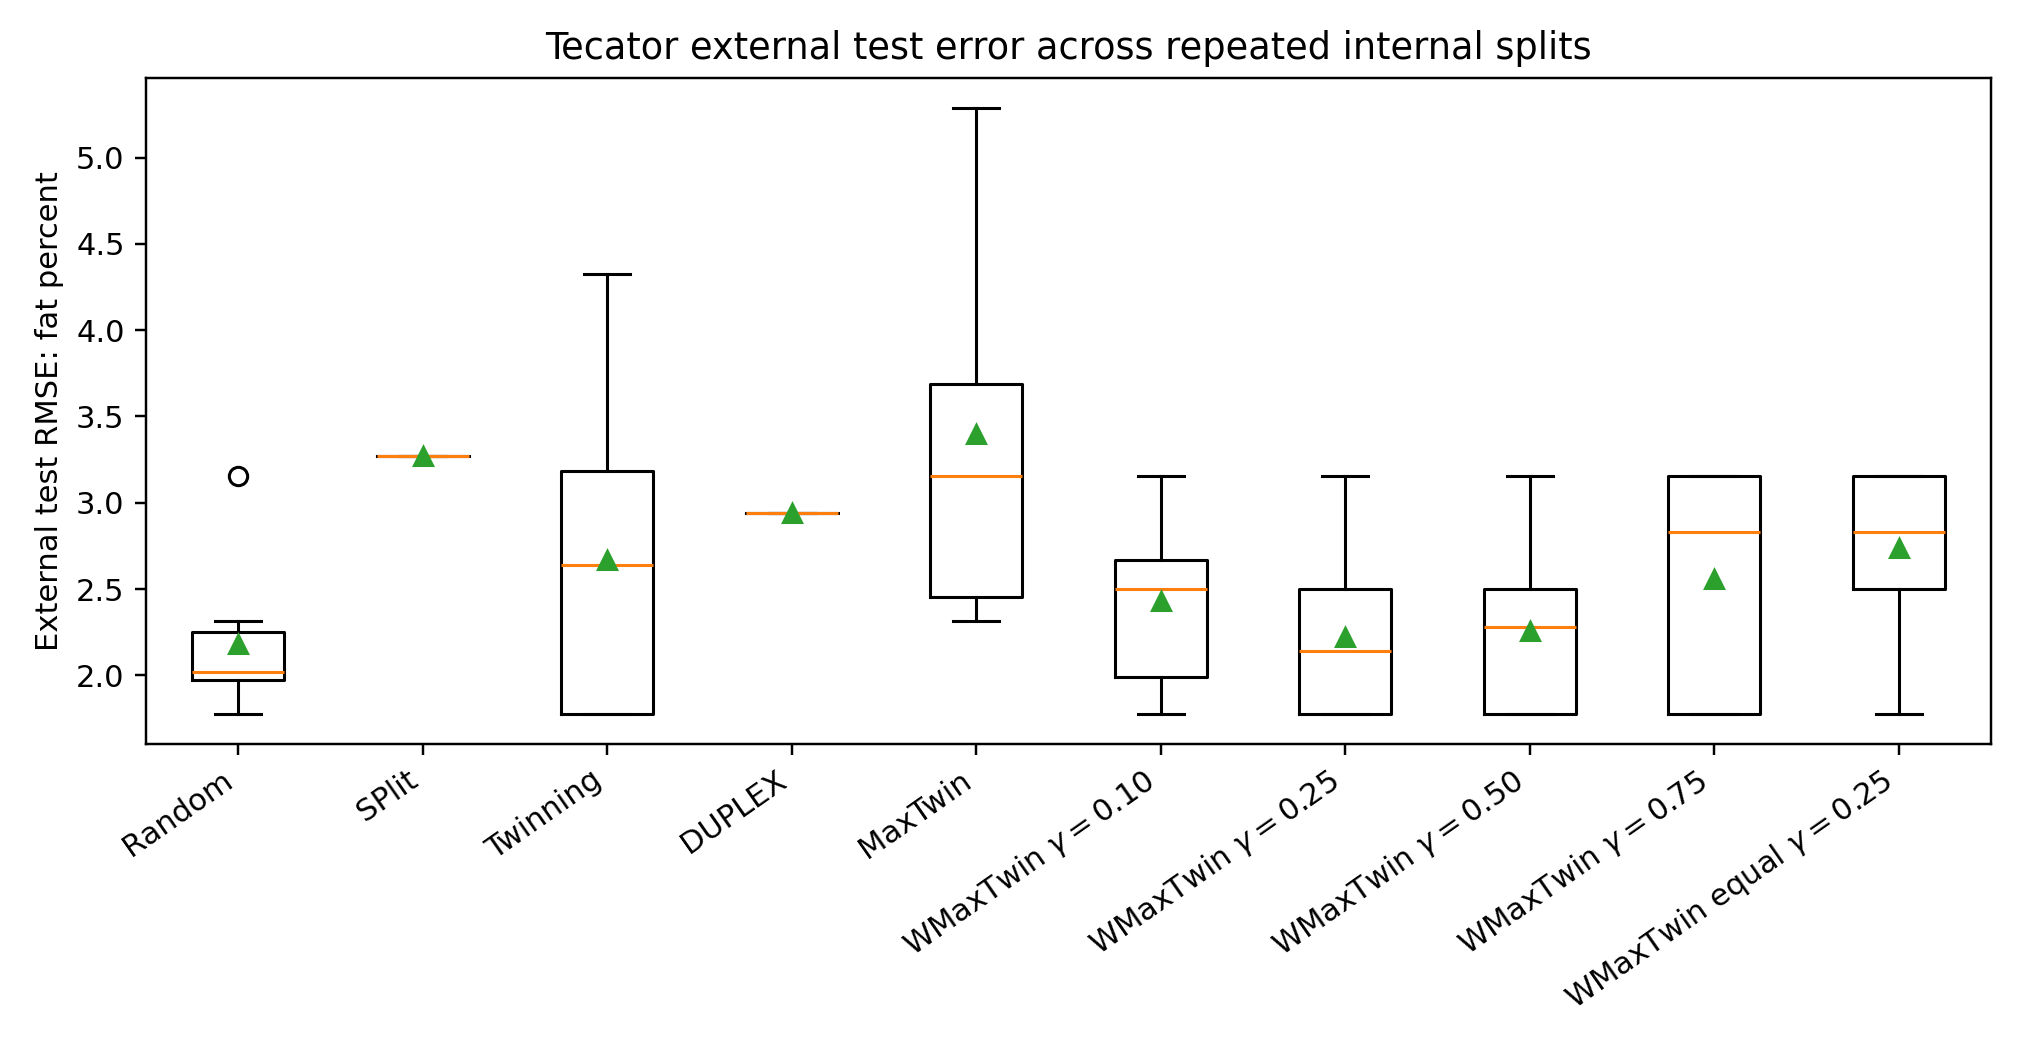
\includegraphics[width=.85\textwidth]{fig5_test_rmse_boxplot.png}
\caption{External test RMSE across repeated internal train-validation splits.}
\label{fig:tecator-rmse}
\end{figure}

\begin{figure}[t]
\centering
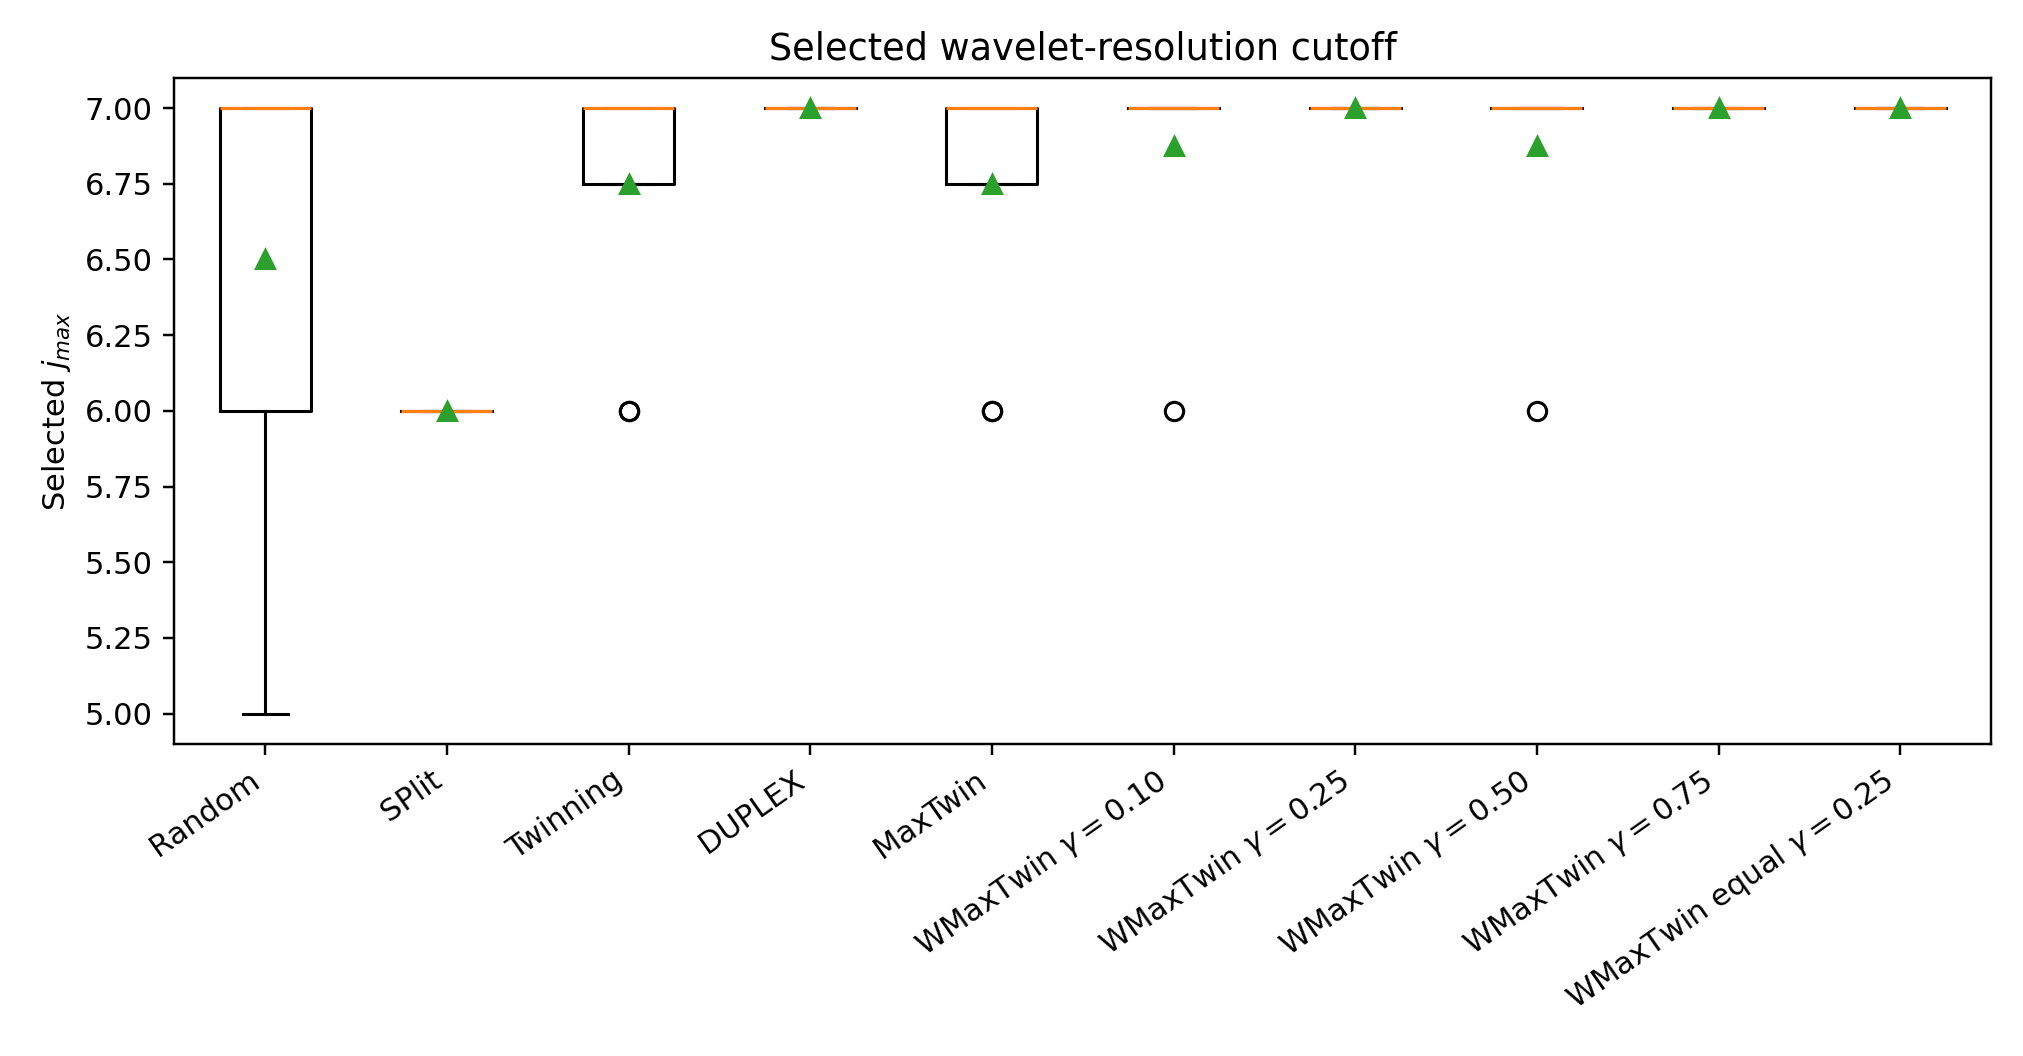
\includegraphics[width=.85\textwidth]{fig6_selected_jmax_boxplot.png}
\caption{Selected wavelet-resolution cutoff across repeated internal splits.}
\label{fig:tecator-jmax}
\end{figure}

\begin{figure}[t]
\centering
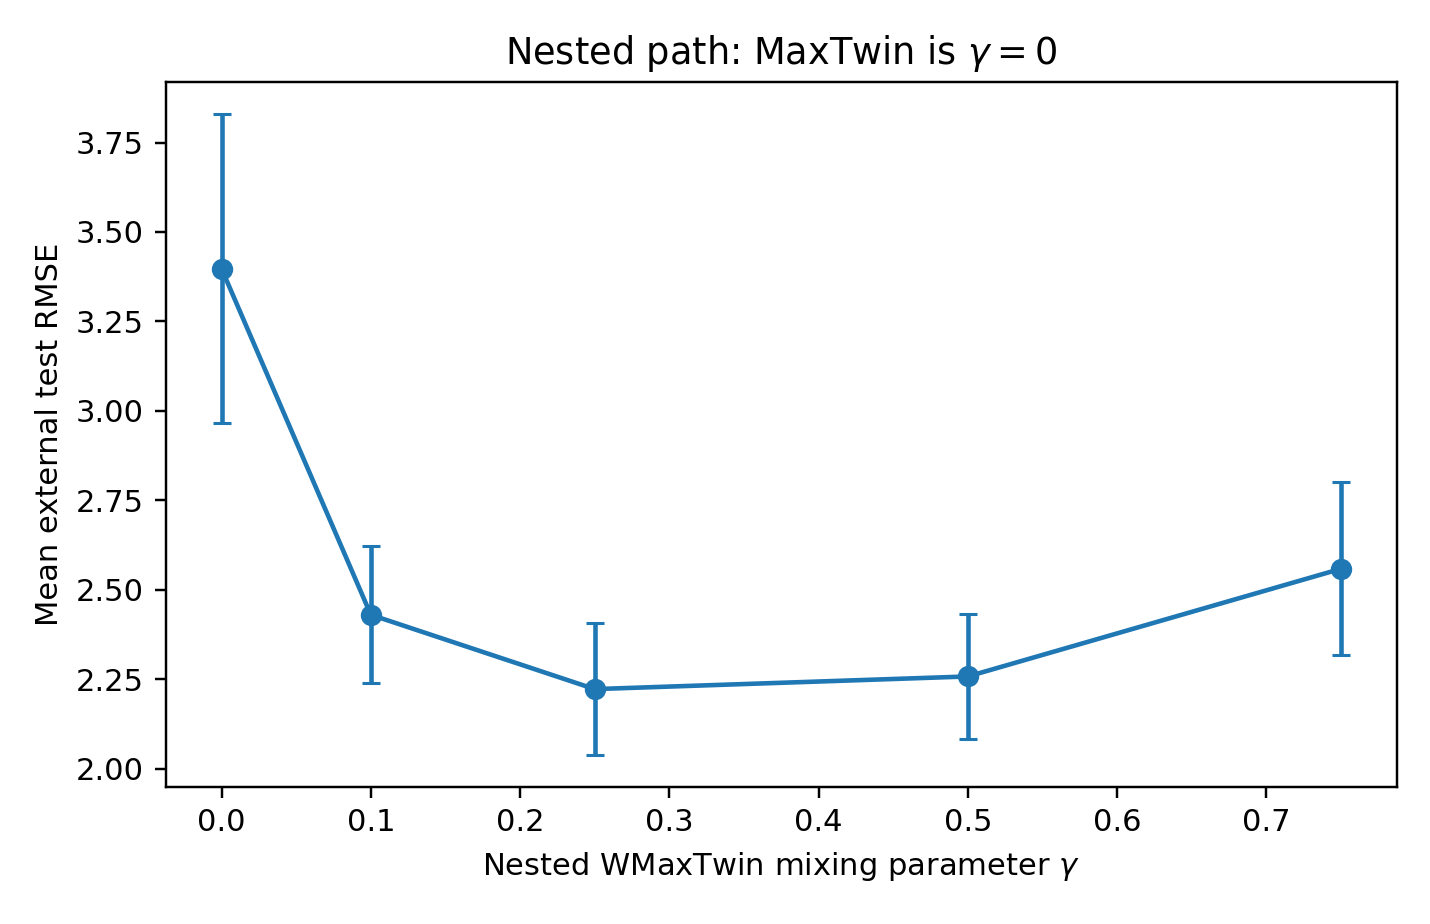
\includegraphics[width=.72\textwidth]{fig8_gamma_path_rmse.png}
\caption{Nested WMaxTwin path.  MaxTwin corresponds to $\gamma=0$; positive
$\gamma$ values add scale-weighted wavelet geometry.}
\label{fig:tecator-gamma}
\end{figure}
